% -*- mode: LaTeX; mode: TeX-PDF; coding: utf-8  -*-

\label{sec:func_recv}

%%%%%%%%%%%%%%%%%%%%%%%%%%%%%%%%%%%%%%%%%%%%%%%%%%%%%%%%%%%%%%%%%
\subsection*{Схема вычислений в модели Open CL}


Введём  следующие обозначения.
\begin{itemize}

\item
  $F$  --- массив  известных значений функции $\varphi$
  в узлах крупной сетки;

\item
  $G_{r+\mathbf{2}^n}$ --- массив
  значений аппроксимирующей функции в узлах мелкой сетки,
  вычисленных по формуле~\eqref{eq:recv_common};

\item
  $\Psi_{r+\mathbf{2}^n}$ --- массив  значений ядер В. А. Стеклова порядка $r+\mathbf{2}^n$.

\end{itemize}

%\emph{согласен что плохо, но непонятно какая концепция у нас}

%Учитывая финитность и симметрию ядер В. А. Стеклова
%в массиве $\Psi_{2}$ нужно хранить $N^*$
%значений ядер $\psi_{2}$;
%%на одном интервале крупной сетки;
%в массиве $\Psi_{4}$ нужно хранить $2N^*$
%значений ядер $\psi_{4}$.
%на двух смежных интервалах крупной сетки.

% Учитывая финитность и симметрию ядер В. А. Стеклова
% в массиве $\Psi_{{r+\mathbf{2}^n}}$ достаточно хранить $\overline{r(N+\mathbf{1}^n)/ 2}$
% значений.

% \emph{Сюда можно вставить рисунок 2D ядра 2го порядка для наглядности.
% Выделить ту четвертинку, которую храним.}
Пример ядра порядка 4 на рисунке, $N=4$.

\begin{figure}[h!]
  \centering
  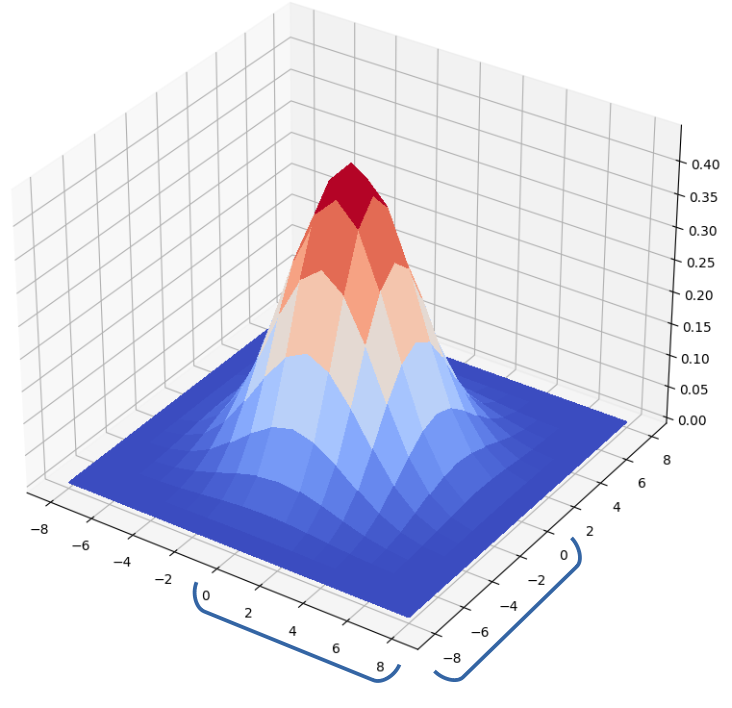
\includegraphics[width=\textwidth
   % ,height
  ]{kern_4_4} 
  \caption{Ядро 4го порядка}
  \label{fig:reg_net}
\end{figure}
\FloatBarrier


 Далее приведены выражения для формирования
 элементов искомых значений в узлах мелкой сетки.
% %,
% \emph{где $n$ -- количество координат (размерность задачи). --- уже раньше использовали}
%\emph{Итоговая формула, м.б. от массивов вернуться к функциям?}
Пусть $m\in M$, тогда
\begin{equation}
  \label{eq:nd}
    G_{r+\mathbf{2}^n}[m] = 
    \sum_{i \in  [\mathbf{0}^n:r/2]}\ \sum_{p\in P} 
        F \left[ \left \lfloor {m}/{N} \right \rfloor + ip + s(p)\right]
      \Psi_{r+\mathbf{2}^n}[|m\bmod N - (pi + s(p))N|],
\end{equation}
где $P=\{p\in\mathbb{Z}^n: p_l\in\{-1,1\},\ l=1,\ldots,n\}$, $s(t)=(t+1)/2$
($t\in\mathbb{R}$).


При вычислениях по формуле~\eqref{eq:nd} требуется
%в двумерном случае (2 - операции * и +, 4 части)
%$2 * 4 * \overline{(r/\mathbf{2}^n+\mathbf{1}^n) M}.$
%в общем случае (2 - операции * и +, $2^n$ частей)
$2^n * \overline{(r/\mathbf{2}^n+\mathbf{1}^n)} \overline{M}$
умножений и
$(2^n-1) * (\overline{(r/\mathbf{2}^n+\mathbf{1}^n)} -1)  \overline{M}$
сложений. 


%По одной координате выражение имеет вид:
% Если $A$ --- $n$-мерный массив, то $[A[i_j]]_j$ означает срез по $j$-й координате, т.~е.
% $A[i_1,\ldots,i_{j-1},i_j,i_{j+1},\ldots,j_n]$, где $i_l$ фиксированы при $l\neq j$.

% \begin{equation}
%   \label{eq:1d}
%   \begin{split}
%     [G_r[m_j]]_{j} &= 
%     \sum_{i = 0}^{r_j/2 +1}
%     \left[
%         F \left[ \left \lfloor {m_j}/{N_j^*} \right \rfloor - i\right]
%     \right]_{j}
%     \left[
%       \Psi_{r+\mathbf{2}^n}[iN_j^* + m_j\bmod N_j^*] 
%     \right]_{j}
%        + \\
%     &  +
%     \left[
%       F \left[\left\lfloor {m_j}/{N_j^*} \right \rfloor + (i+1) \right]
%     \right]_{j}
%     \left[
%       \Psi_{r+\mathbf{2}^n}[(i+1)N_j^* - m_j \bmod N_j^*]
%     \right]_{j}
%   \end{split}
% \end{equation}

\begin{comment}
\emph{Двумерный случай:}

\begin{equation*}
  \begin{split}
    G_r[m_1,m_2] &= 
    \sum_{i_1 = 0}^{r_1/2 +1} \sum_{i_2 = 0}^{r_2/2 +1}
        F \left[ \left \lfloor {m_1}/{N_1} \right \rfloor - i_1, \left \lfloor {m_2}/{N_2} \right \rfloor - i_2\right]
      \Psi_{r_1+2,r_2+2}[i_1N_1 + m_1\bmod N_1,i_2N_2 + m_2\bmod N_2] 
       + \\
    &  +
      F \left[\left\lfloor {m_1}/{N_1} \right \rfloor + (i_1+1), \left\lfloor {m_2}/{N_2} \right \rfloor + (i_2+1)  \right]
      \Psi_{r_1+2,r_2+2}[(i_1+1)N_1 - m_1 \bmod N_1,(i_2+1)N_2 - m_2 \bmod N_2]
  \end{split}
\end{equation*}
  
\end{comment}


Иллюстрация при $r=2$ суммирования по одной координате на рисунке.
\begin{figure}[h!]
  \centering
  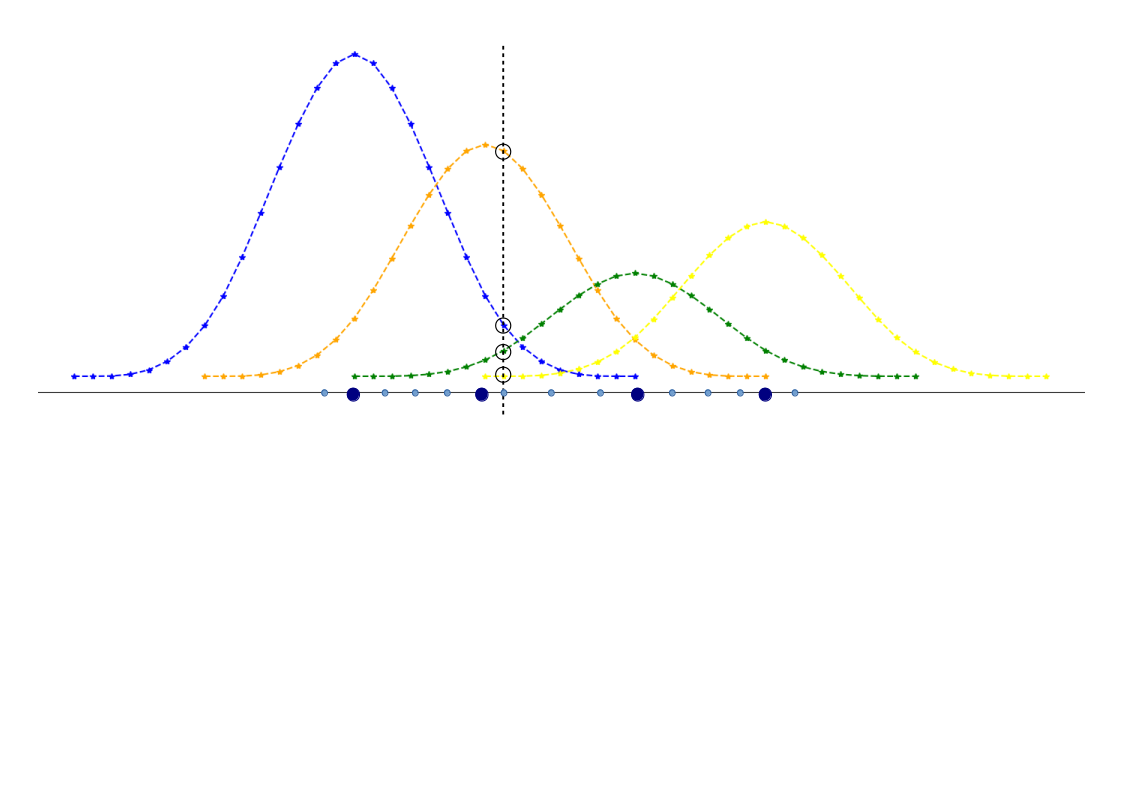
\includegraphics[width=\textwidth,height=7cm]{multi_kern} 
  \caption{пример для одной координаты}
  \label{fig:reg_net}
\end{figure}
\FloatBarrier



% Заметка про этапы индексации.
% \emph{Можно как=то учесть в обозначениях}
% \begin{enumerate}
% \item
%   Лоцировать ячейку в которой находится искомая точка мелкой сетки.
%   Операция $\left \lfloor \frac{m_j}{N_j^*} \right \rfloor$.

% \item
%   Отобразить индекс в координатах всей мелкой сетки на координаты в ячейке.
%   Операция $m_j \bmod N_j^*$.
% \end{enumerate}
  


%%

Заметим, 
что в формуле~\eqref{eq:nd} каждое из произведений известного значения в узле крупной сетки
со значениями ядер в узлах мелкой сетки используется несколько раз
при формировании результатов в нескольких соседних
%интервалах
ячейках 
крупной сетки. 
С учётом этого факта,
предложена следующая двухэтапная вычислительная схема.
\begin{enumerate}
\item
  %Вычисление произведений значений ядер в узлах мелкой сетки
  %для каждого узла крупной сетки.
  Вычисление для $k$-го ($k \in [0:K-\mathbf{1}^n]$)
  известного значения функции 
  элементов массива произведений
  $\Pi_r[k,l] = F[k]\Psi_{r+\mathbf{2}^n}[l]$,
($l \in [0:(r/2+\mathbf{1}^n)(N-\mathbf{1}^n)]$).
  %($l \in [0:r(N-\mathbf{1}^n)/2]$).
  Выполняется %$\overline{K(rN)/2}$
  $\overline{K(r/2+\mathbf{1}^n)N}$ умножений.
  %$\prod_{i=1}^n K_i(r_iN_i)/2^n$ 

  Выполняется $\overline{K (N(r/\mathbf{2}^n + \mathbf{1}^n) +\mathbf{1}^n)}$ умножений.

\item
  Выбор и суммирование полученных на предыдущем шаге произведений
  для формирования результирующих значений в узлах мелкой сетки.
  
  %Выполняется $r^2M$ сложений.
  %$M$ сложений в первом варианте и
  %$3M$ сложений --- во втором.

  Выполняется $(2^n-1) * (\overline{(r/\mathbf{2}^n+\mathbf{1}^n)} -1)  \overline{M}$ сложений.

\end{enumerate}

Таким образом за счёт переиспользования произведений при применении вычислительной схемы
количество умножений сокращается почти в  $2^n$ раз.

%При такой схеме вычислений общее количество арифметических операций
%для восстановления данных без сглаживания
%составляет $2KN + 2K - N$ (что меньше, чем $3M = 3NK + 3K - 3N$)
%и $5KN + 5K - 3N$ (что меньше, чем $7M = 7NK + 7K - 7N$) для
%восстановления данных со сглаживанием.

%Задача восстановления данных в узлах мелкой сетки
%рассматривается как одна стадия конвейера в модели БСКП.
%ВПД этой стадии является массив $F$ размером $K$,
%содержащий известные
%значения в узлах крупной сетки.
%Обработка ВПД  %восстановления значений в узлах мелкой сетки
%состоит из двух вычислительных процедур,
%соответствующих перечисленным выше этапам.


Иллюстрация вычислительной схемы на рисунке.
\begin{figure}[h!]
  \centering
  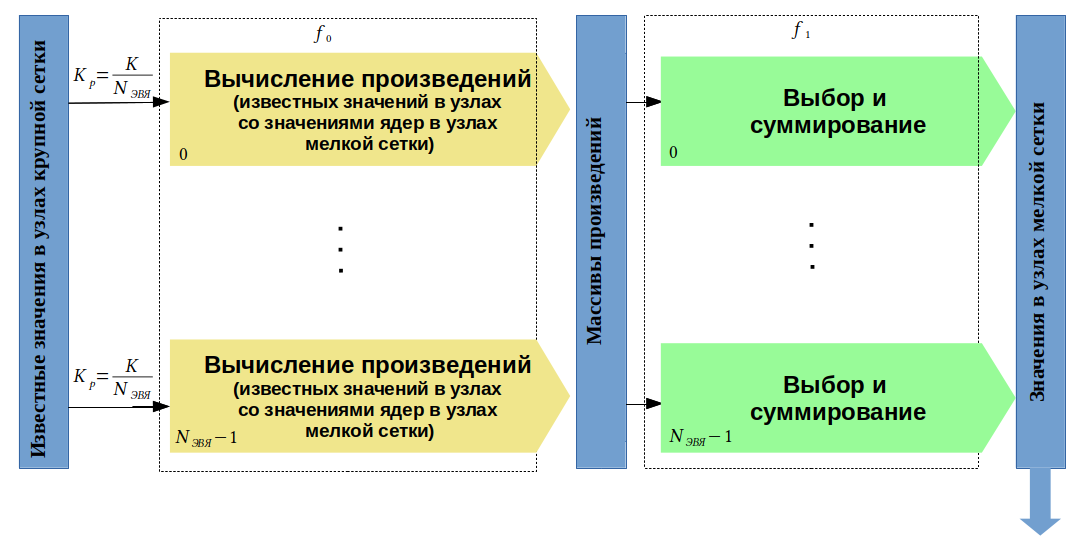
\includegraphics[width=\textwidth,height=7cm]{comp_scheme_steps} 
  \caption{Двухэтапная вычислительная схема}
  \label{fig:reg_net}
\end{figure}
\FloatBarrier

\subsection*{Схема вычислений в модели Open CL}


Введём  следующие обозначения.
\begin{itemize}

\item
  $F$  --- массив  известных значений функции $\varphi$
  в узлах крупной сетки;

\item
  $G_{r+\mathbf{2}^n}$ --- массив
  значений аппроксимирующей функции в узлах мелкой сетки,
  вычисленных по формуле~\eqref{eq:recv_common};

\item
  $\Psi_{r+\mathbf{2}^n}$ --- массив  значений ядер В. А. Стеклова порядка $r+\mathbf{2}^n$.

\end{itemize}

%\emph{согласен что плохо, но непонятно какая концепция у нас}

%Учитывая финитность и симметрию ядер В. А. Стеклова
%в массиве $\Psi_{2}$ нужно хранить $N^*$
%значений ядер $\psi_{2}$;
%%на одном интервале крупной сетки;
%в массиве $\Psi_{4}$ нужно хранить $2N^*$
%значений ядер $\psi_{4}$.
%на двух смежных интервалах крупной сетки.

% Учитывая финитность и симметрию ядер В. А. Стеклова
% в массиве $\Psi_{{r+\mathbf{2}^n}}$ достаточно хранить $\overline{r(N+\mathbf{1}^n)/ 2}$
% значений.

% \emph{Сюда можно вставить рисунок 2D ядра 2го порядка для наглядности.
% Выделить ту четвертинку, которую храним.}
Пример ядра порядка 4 на рисунке, $N=4$.

\begin{figure}[h!]
  \centering
  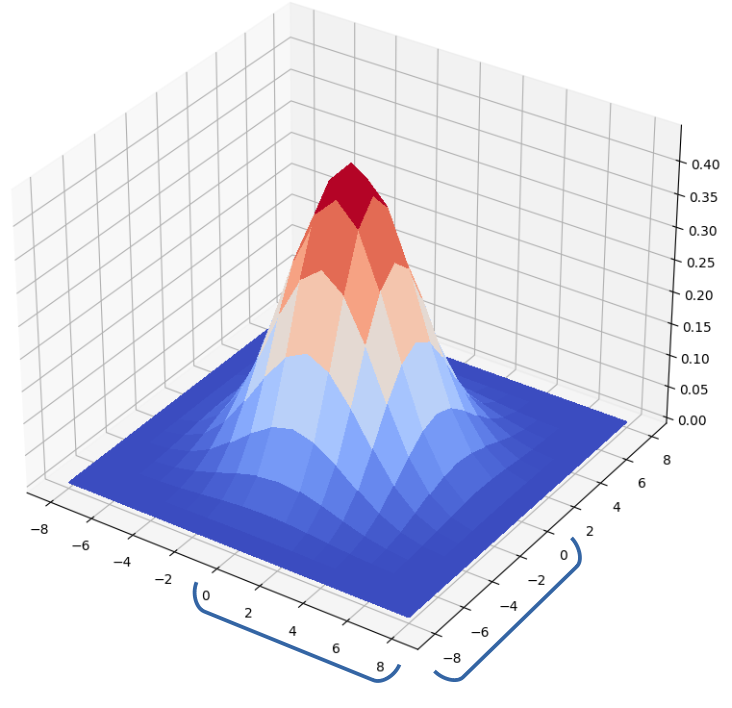
\includegraphics[width=\textwidth
   % ,height
  ]{kern_4_4} 
  \caption{Ядро 4го порядка}
  \label{fig:reg_net}
\end{figure}
\FloatBarrier


 Далее приведены выражения для формирования
 элементов искомых значений в узлах мелкой сетки.
% %,
% \emph{где $n$ -- количество координат (размерность задачи). --- уже раньше использовали}
%\emph{Итоговая формула, м.б. от массивов вернуться к функциям?}
Пусть $m\in M$, тогда
\begin{equation}
  \label{eq:nd}
    G_{r+\mathbf{2}^n}[m] = 
    \sum_{i \in  [\mathbf{0}^n:r/2]}\ \sum_{p\in P} 
        F \left[ \left \lfloor {m}/{N} \right \rfloor + ip + s(p)\right]
      \Psi_{r+\mathbf{2}^n}[|m\bmod N - (pi + s(p))N|],
\end{equation}
где $P=\{p\in\mathbb{Z}^n: p_l\in\{-1,1\},\ l=1,\ldots,n\}$, $s(t)=(t+1)/2$
($t\in\mathbb{R}$).


При вычислениях по формуле~\eqref{eq:nd} требуется
%в двумерном случае (2 - операции * и +, 4 части)
%$2 * 4 * \overline{(r/\mathbf{2}^n+\mathbf{1}^n) M}.$
%в общем случае (2 - операции * и +, $2^n$ частей)
$2^n * \overline{(r/\mathbf{2}^n+\mathbf{1}^n)} \overline{M}$
умножений и
$(2^n-1) * (\overline{(r/\mathbf{2}^n+\mathbf{1}^n)} -1)  \overline{M}$
сложений. 


%По одной координате выражение имеет вид:
% Если $A$ --- $n$-мерный массив, то $[A[i_j]]_j$ означает срез по $j$-й координате, т.~е.
% $A[i_1,\ldots,i_{j-1},i_j,i_{j+1},\ldots,j_n]$, где $i_l$ фиксированы при $l\neq j$.

% \begin{equation}
%   \label{eq:1d}
%   \begin{split}
%     [G_r[m_j]]_{j} &= 
%     \sum_{i = 0}^{r_j/2 +1}
%     \left[
%         F \left[ \left \lfloor {m_j}/{N_j^*} \right \rfloor - i\right]
%     \right]_{j}
%     \left[
%       \Psi_{r+\mathbf{2}^n}[iN_j^* + m_j\bmod N_j^*] 
%     \right]_{j}
%        + \\
%     &  +
%     \left[
%       F \left[\left\lfloor {m_j}/{N_j^*} \right \rfloor + (i+1) \right]
%     \right]_{j}
%     \left[
%       \Psi_{r+\mathbf{2}^n}[(i+1)N_j^* - m_j \bmod N_j^*]
%     \right]_{j}
%   \end{split}
% \end{equation}

\begin{comment}
\emph{Двумерный случай:}

\begin{equation*}
  \begin{split}
    G_r[m_1,m_2] &= 
    \sum_{i_1 = 0}^{r_1/2 +1} \sum_{i_2 = 0}^{r_2/2 +1}
        F \left[ \left \lfloor {m_1}/{N_1} \right \rfloor - i_1, \left \lfloor {m_2}/{N_2} \right \rfloor - i_2\right]
      \Psi_{r_1+2,r_2+2}[i_1N_1 + m_1\bmod N_1,i_2N_2 + m_2\bmod N_2] 
       + \\
    &  +
      F \left[\left\lfloor {m_1}/{N_1} \right \rfloor + (i_1+1), \left\lfloor {m_2}/{N_2} \right \rfloor + (i_2+1)  \right]
      \Psi_{r_1+2,r_2+2}[(i_1+1)N_1 - m_1 \bmod N_1,(i_2+1)N_2 - m_2 \bmod N_2]
  \end{split}
\end{equation*}
  
\end{comment}


Иллюстрация при $r=2$ суммирования по одной координате на рисунке.
\begin{figure}[h!]
  \centering
  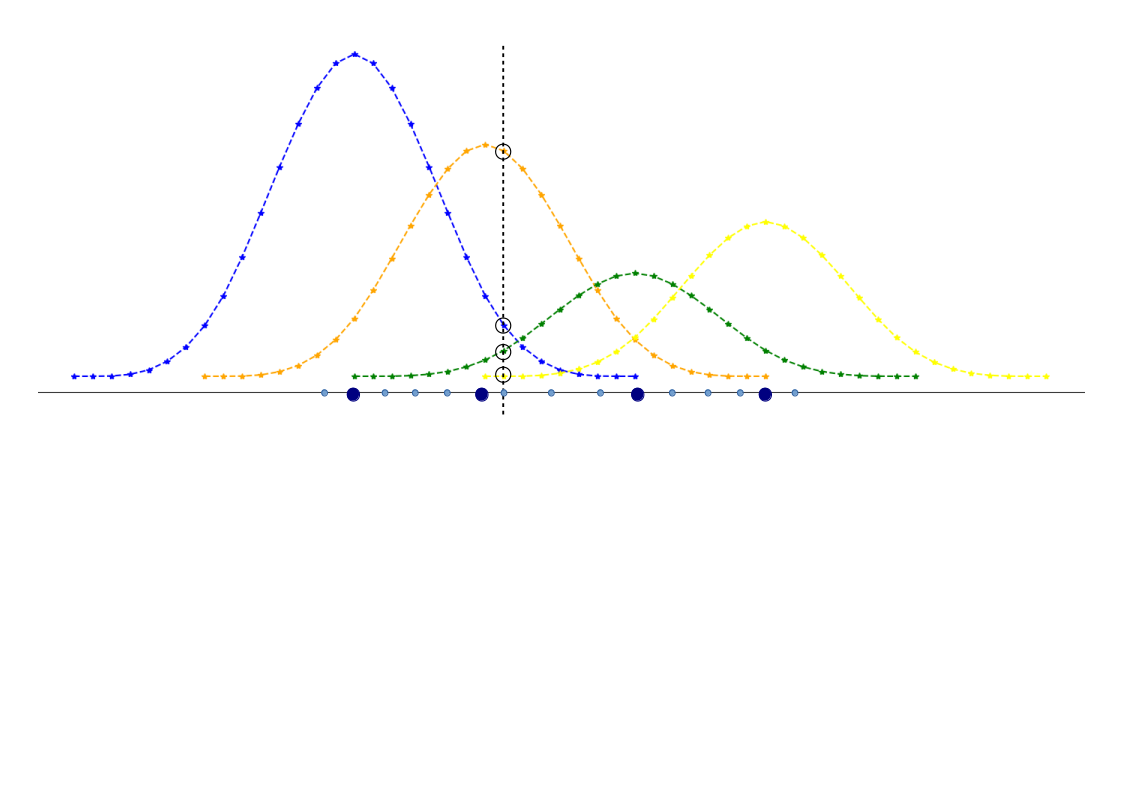
\includegraphics[width=\textwidth,height=7cm]{multi_kern} 
  \caption{пример для одной координаты}
  \label{fig:reg_net}
\end{figure}
\FloatBarrier



% Заметка про этапы индексации.
% \emph{Можно как=то учесть в обозначениях}
% \begin{enumerate}
% \item
%   Лоцировать ячейку в которой находится искомая точка мелкой сетки.
%   Операция $\left \lfloor \frac{m_j}{N_j^*} \right \rfloor$.

% \item
%   Отобразить индекс в координатах всей мелкой сетки на координаты в ячейке.
%   Операция $m_j \bmod N_j^*$.
% \end{enumerate}
  


%%

Заметим, 
что в формуле~\eqref{eq:nd} каждое из произведений известного значения в узле крупной сетки
со значениями ядер в узлах мелкой сетки используется несколько раз
при формировании результатов в нескольких соседних
%интервалах
ячейках 
крупной сетки. 
С учётом этого факта,
предложена следующая двухэтапная вычислительная схема.
\begin{enumerate}
\item
  %Вычисление произведений значений ядер в узлах мелкой сетки
  %для каждого узла крупной сетки.
  Вычисление для $k$-го ($k \in [0:K-\mathbf{1}^n]$)
  известного значения функции 
  элементов массива произведений
  $\Pi_r[k,l] = F[k]\Psi_{r+\mathbf{2}^n}[l]$,
($l \in [0:(r/2+\mathbf{1}^n)(N-\mathbf{1}^n)]$).
  %($l \in [0:r(N-\mathbf{1}^n)/2]$).
  Выполняется %$\overline{K(rN)/2}$
  $\overline{K(r/2+\mathbf{1}^n)N}$ умножений.
  %$\prod_{i=1}^n K_i(r_iN_i)/2^n$ 

  Выполняется $\overline{K (N(r/\mathbf{2}^n + \mathbf{1}^n) +\mathbf{1}^n)}$ умножений.

\item
  Выбор и суммирование полученных на предыдущем шаге произведений
  для формирования результирующих значений в узлах мелкой сетки.
  
  %Выполняется $r^2M$ сложений.
  %$M$ сложений в первом варианте и
  %$3M$ сложений --- во втором.

  Выполняется $(2^n-1) * (\overline{(r/\mathbf{2}^n+\mathbf{1}^n)} -1)  \overline{M}$ сложений.

\end{enumerate}

Таким образом за счёт переиспользования произведений при применении вычислительной схемы
количество умножений сокращается почти в  $2^n$ раз.

%При такой схеме вычислений общее количество арифметических операций
%для восстановления данных без сглаживания
%составляет $2KN + 2K - N$ (что меньше, чем $3M = 3NK + 3K - 3N$)
%и $5KN + 5K - 3N$ (что меньше, чем $7M = 7NK + 7K - 7N$) для
%восстановления данных со сглаживанием.

%Задача восстановления данных в узлах мелкой сетки
%рассматривается как одна стадия конвейера в модели БСКП.
%ВПД этой стадии является массив $F$ размером $K$,
%содержащий известные
%значения в узлах крупной сетки.
%Обработка ВПД  %восстановления значений в узлах мелкой сетки
%состоит из двух вычислительных процедур,
%соответствующих перечисленным выше этапам.


Иллюстрация вычислительной схемы на рисунке.
\begin{figure}[h!]
  \centering
  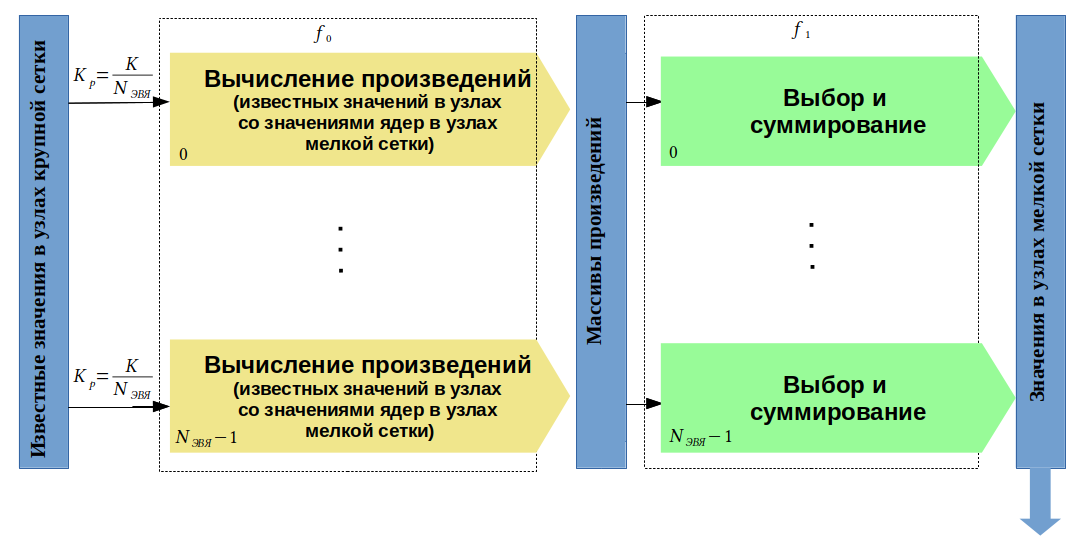
\includegraphics[width=\textwidth,height=7cm]{comp_scheme_steps} 
  \caption{Двухэтапная вычислительная схема}
  \label{fig:reg_net}
\end{figure}
\FloatBarrier


\subsection*{Реализация двумерного случая}

Из RAM управляющего процессора
в VRAM вычислительного ускорителя
загружаются следующие данные: 
\begin{itemize}
\item
  Массив значений в узлах крупной сетки. %размером $K = K_y*K_x$.
\item
  Массив значений ядра порядка $r$. %, вычисленных в $(r/2)^2$ ячейках мелкой сетки.
  C учётом финитности ядна и его симметричности по
  обом координатам хранить достаточно одну четверть.
  Инициализируется предварительно.
\end{itemize}

Результирующие значения в узлах мелкой сетки выгружаются управляющим процессором
из VRAM по завершению работы вычислительных ядер на ускорителе.

Программная реализация рассмотренного алгоритма в двухмерном случае
включает в себя 2 вычислительных ядра, соответствующие этапам схемы вычислений.
Первое вычислительное ядро выполняется в размерности рабочего пространства $K$,
для второго удобно выбрать размерность $M$.
Далее приведено описание, разработаных вычислительных ядрер.
\begin{itemize}
\item
  {\bf kernel prod}

  Выполняется в каждой точке крупной сетки.
  Каждый вычислительны элемент 
  получает точку крупной сетки
  из VRAM по $globalID$. 
  
  %Размер задачи $K$ (оно же
  %максимальное количество параллельно выполняющихся kernel prod).
  %Размер задачи для этого ядра одномерный (но мб двумерным сделать для наглядности).

  На выходе в VRAM
  формируются массивы произведений в $(r/2)^2$ ячейках мелкой сетки  
  соответствующие каждой точке крупной сетки.
%Выходная структура данных типа map --- для взаимно однозначного соответствия точка -> массив произведений в ячейках.

  
\item
  {\bf kernel sum}

  Суммирует $r$ ближайших по каждой координате к $globalID$ произведений. 
  Выполняется в каждой точке мелкой сетки.
  
  
  Каждый вычислительный элемент записывает свою точку мелкой сетки в
  массив в VRAM по GlobalID
\end{itemize}



%%% Local Variables: 
%%% mode: latex
%%% TeX-master: "paper_func_recv"
%%% End: 



